\documentclass[UTF8,fontset=windowsnew]{ctexart}
\usepackage{amsmath}
\DeclareMathOperator*{\uint}{\scalerel*{\rotatebox{8}{$\!\scriptstyle\int\!$}}{\int}}
  \usepackage{scalerel}
\usepackage{hyperref}
\usepackage{graphicx}
\usepackage{xcolor}
\usepackage[left=2cm,right=2cm, top=2cm, bottom=2cm]{geometry}
\usepackage{fancyhdr}
  \pagestyle{fancy}
  \fancyhf{}
  \rhead{\large{\emph{考核系统}}}
  \setlength{\headheight}{20pt}
  \rfoot{\thepage}
\usepackage{enumitem}
\usepackage{tikz}
  \newcommand*\circled[1]{\tikz[baseline=(char.base)]{\node[shape=circle,draw,inner sep=2pt] (char) {#1};}}
  \newcommand{\RomanNumeralCaps}[1]{\MakeUppercase{\romannumeral #1}}
\usepackage{multicol}

\begin{document}
\songti

\section{需求}
\subsection{原始需求}
需要对每个被考核人进行工作量计算。
\begin{enumerate}[label=\protect\circled{\arabic*}]
    \item 工作量计算
    \item 计算过程图像化展示
    \item 用户管理
\end{enumerate}
\subsection{需求分析}
\subsubsection{工作量计算}
\begin{equation}
  C=\frac{1}{N}\sum_{i-1}^NC_i\label{eq:main}
\end{equation}
$C_i=\frac{W_i}{S_i}$为总工作量,$N$为考核项目数量,$W_i$为考核项目完成量,$S_i$为标准任务量。\par
\subsubsection{图像化展示}
将各项参数的组成部分图像化
\subsubsection{用户管理}
允许被考核人亲自上传各个表格
\section{被考核人}
被考核人应由工号辨别,如允许以姓名辨别,应处理重名。\par
每个被考核人属于一种岗位类型:\par
\begin{itemize}
  \item 教学科研岗
  \item 教学岗
  \item 科研岗
\end{itemize}
每个岗位类型分10级,不同等级对应不同的基准工作量和总任务量。
\section{工作量计算标准}
每种考核方向的比重相同,以恰好完成基准工作量为1,如必要项未完成,为0;如非必要项未完成,按比例扣分;如超标完成,按比例加分。\par
完成每种考核后按\autoref{eq:main}计算总分。\par
\section{产品介绍}
由于工期原因,仅需求\circled{1}可以保证完成;如一切顺利,需求\circled{2}可以数字的形式显示,图像化无法完成;需求\circled{3}确定无法按期完成。\par
\subsubsection{基本架构}
\begin{figure}[h]
  \centering
  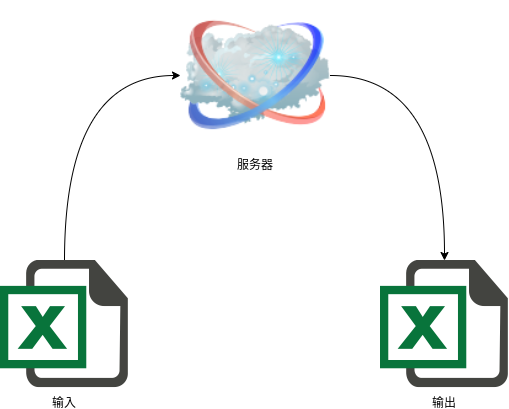
\includegraphics[width=.5\textwidth]{image/struc.png}
  \caption{基本架构}
  \label{fig:struc}
\end{figure}
如\autoref{fig:struc}所示,本产品的基本模式为服务器-客户端模式。\par
\subsection{服务器}
服务器采用Node.js/Express.js/Pug技术,可在Windows/Linux平台上运行。\par
服务器的运行依赖于Nodejs和npm。\par
默认端口为10000。\par
如果需要,可以提供服务器的源代码。\par
测试服务器的地址为\url{http://34.94.165.54:10000/}\par
测试服务器预计可以提供服务到2020年9月。期间如果系统出问题可以保证24小时内解决。
\subsection{客户端}
本产品的客户端为任何浏览器,支持IE 8+, Chrome, Firefox等主流浏览器。如果网页显示出现问题建议更换浏览器后重试。\par
界面:\par
\begin{figure}[h]
  \centering
  
\includegraphics[width=.5\textwidth]{image/client.png}
  \caption{主页面}
  \label{fig:client}
\end{figure}
如\autoref{fig:client}所示,主界面从上到下拥有6个链接。\par
\begin{itemize}
  \setlength{\itemindent}{4em}
  \item [使用本系统前请阅读此文] 该项为本文的链接
  \item [锁定] 点击该项会生成一个上传码
  \item [选择表格] 点击该项会弹窗,请选择需要上传的表格
  \item [上传表格] 点击该按钮会上传输入表格并开始计算。
  \item [下载最新表格] 点击该项会下载最新的输出表格,同时也可作为下一次上传的输入表格。
  \item [下载模板表格] 点击该项会下载模板输入表格,请根据模板表格的结构修改输入数据
\end{itemize}
\subsection{输入}
需要更新数据时首先点击``锁定''按钮获取上传码。如果成功获取,此时其他人不被允许上传新的表格。\par
然后点击``下载最新版表格'',将其中的数据做更改后点击``选择表格''选中更新后的表格。\par
最后点击``上传表格''按钮,在弹窗中输入第一步获取的上传码,点击``确定''后开始上传新表格。\par
稍等10秒后会弹窗告知数据更新的结果,如显示``上传成功''则完成数据的更新,如计算出错或输入数据不全,也会弹窗告知,请耐心等待10秒。\par
此时点击``下载最新版表格''则可获取计算结果。\par
\begin{figure}[h]
  \centering
  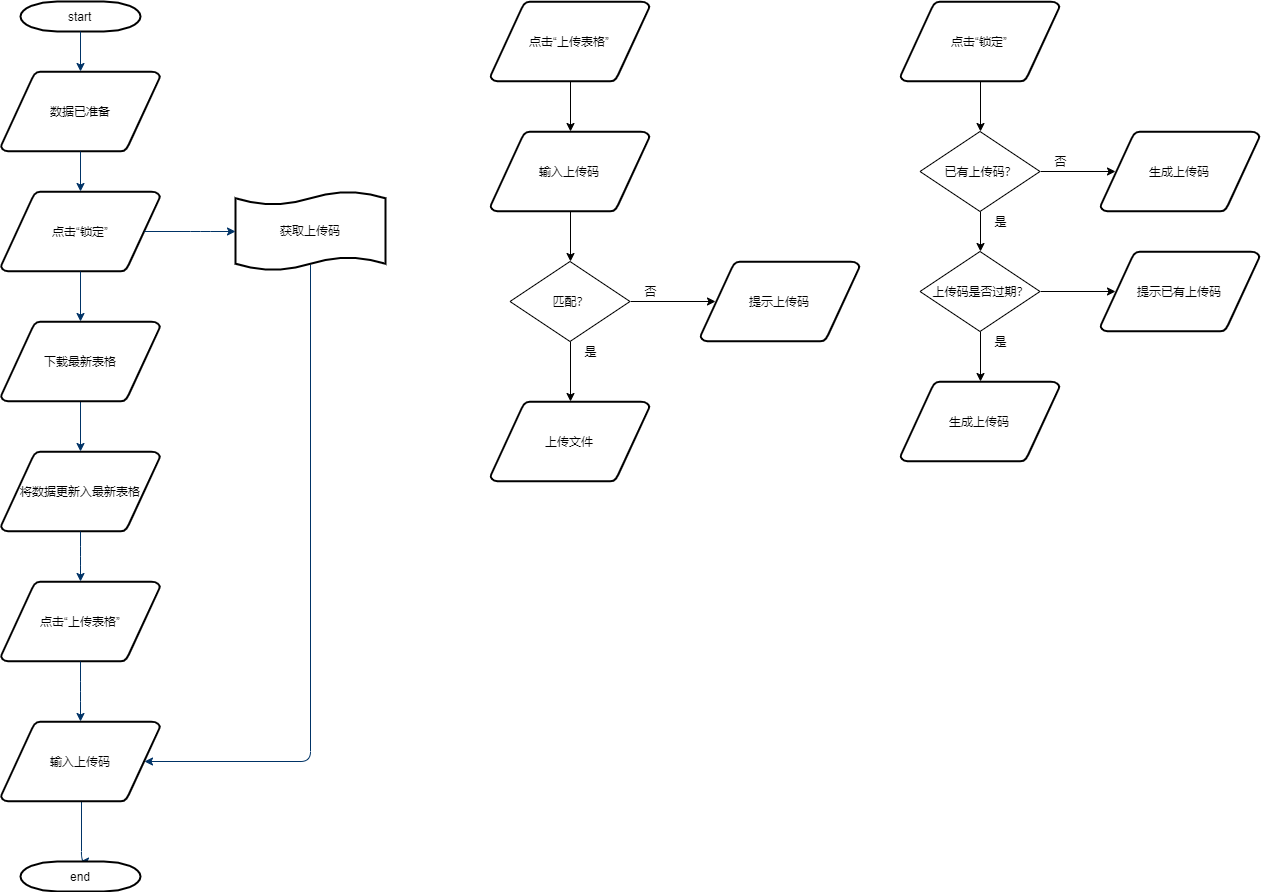
\includegraphics[width=.8\textwidth]{image/lock.png}
  \caption{推荐的更新数据流程}
  \label{fig:lock}
\end{figure}
\autoref{fig:lock}为更新数据时的逻辑流程图。设计此流程的初衷是:假设A和B同时下载了表格,分别修改其中不同的部分,又同时修改完成并上传,此时服务器上就只有A和B其中一人的版本,另一个版本就被覆盖丢失了。\par
通过\autoref{fig:lock}的流程,当A和B同时更新数据时,仅有一人可以获得上传码,因此另一人就知道此时有人正在更新表格。此时就必须等待此次更新完成。\par
当获得上传码的人忘记上传码时,仍可通过点击``锁定''按钮强行获得上传码。若非忘记上传码,不建议强行获取上传码。\par
上传码有效期30分钟,过期就必须重新锁定并获取新的上传码。\par
\url{http://34.94.165.54:10000/template}为模板输入文件。其中有13个表格。每个表格有若干列数据列。数据列以外的列不会影响计算,可以随意编辑。\par
数据列第一行不允许改动,否则系统无法识别数据。其它列没有限制。\par
数据列每一列皆有特定的规范,具体请见模板中每一页的注释。
\subsection{输出}
点击主界面上的``下载最新版表格''可开始下载最新的计算结果。
\begin{figure}[h]
  \centering
  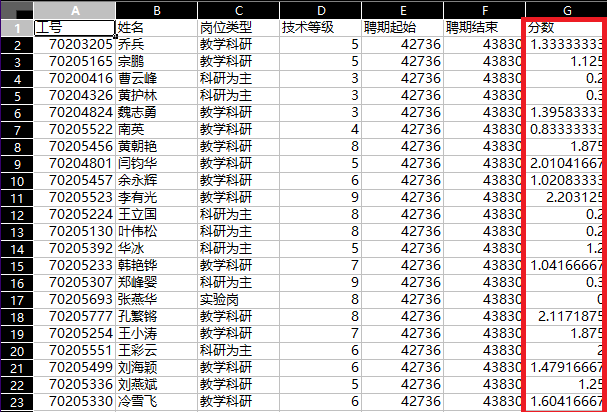
\includegraphics[width=.5\textwidth]{image/output.png}
  \caption{输出范例}
  \label{fig:output}
\end{figure}
\section{缺点}
由于教学为主的老师只有一位,其分数组成又和其他类型的老师差别很大,因此其算法很可能错误。请手动计算其分数。\par
所有团体活动的分数均设为1。如果有详细数据请提供。\par
未纳入班主任和课程设计数据,请手动将其折算并填入本科教学表格。\par
\end{document}
